\section{Introduction to heaps}
\label{sec:introduction_to_heaps}

\begin{frame}
	\frametitle{Heaps}
	\framesubtitle{XKCD Tree: \url{https://xkcd.com/835}}
	\begin{center}
		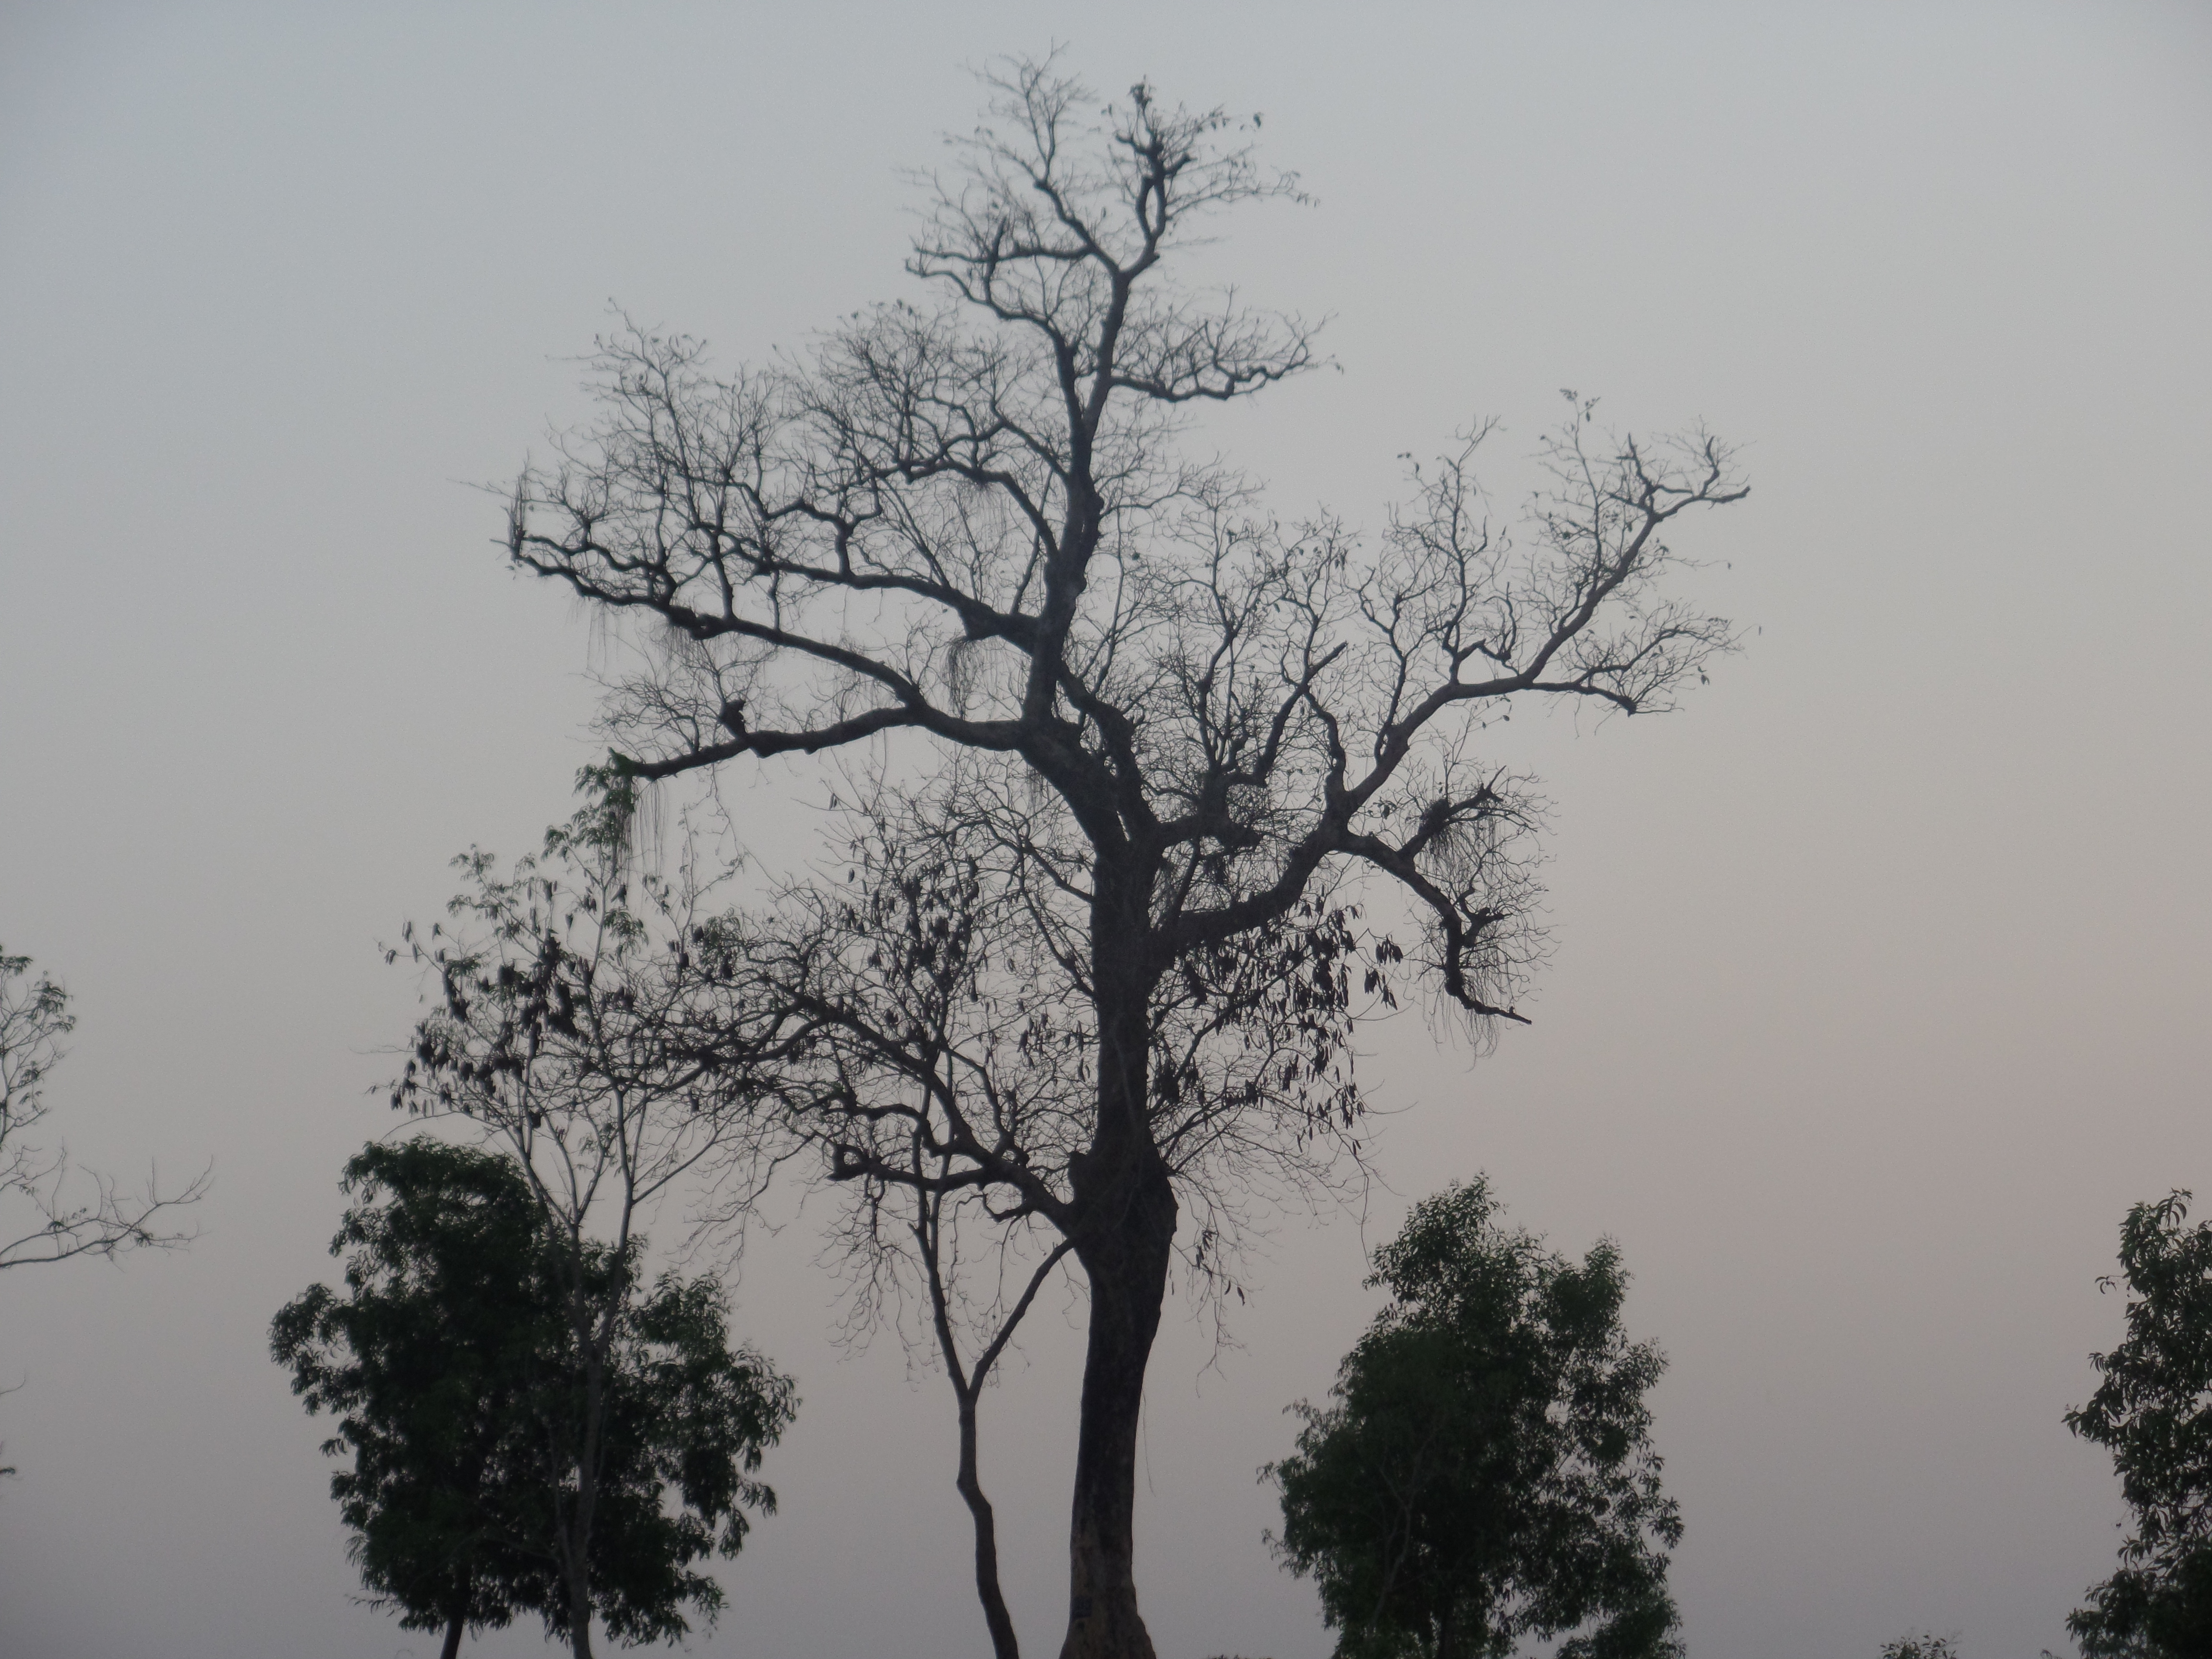
\includegraphics[width=0.6\textwidth]{figures/tree.png}\\
	\end{center}
\end{frame}

\begin{frame}
	\frametitle{Heaps}
		\begin{block}{Heaps}
			We impose extra constraints and create a \textit{heap}:
			\begin{itemize}
				\item \textbf{Heap-order property:} For all nodes: The item stored in a node is greater than the item stored in its parent.
				\item \textbf{Complete Binary Tree property:} The tree is \textit{complete}: Meaning all layers are full, except possibly the last one which has only
					nodes in the left-most positions. 
			\end{itemize}
			\pause
			In this way, it is called a \textit{min-heap}. A \textit{max-heap} has the largest key in the root.
		\end{block}	
		\pause
		\begin{columns}
			\column{0.455\textwidth}

			\begin{tikzpicture}[
				level distance = 2.5em,
				level 1/.style={sibling distance=9em},
				level 2/.style={sibling distance=4.5em},
				level 3/.style={sibling distance=2.25em},
				]
				\node[ellipse] (t1) {1}
				child { node[ellipse]   {12}
					child { node[ellipse] {14}}
				}
				child { node[ellipse]   {4}
					child { node[ellipse] {5}}
					child { node[ellipse] {17}}
				};
			\end{tikzpicture}
			\column{0.455\textwidth}

			\begin{questionblock}{Is it full?}
				Is this a correct min-heap?
			\end{questionblock}
			\pause
			\vspace{-10pt}
			\begin{alertblock}{Nope}
				No, as we do not use the left-most spots in the bottom layer.
			\end{alertblock}
		\end{columns}
\end{frame}

\begin{frame}
	\frametitle{A use case}
	\framesubtitle{Me and my books, part 3}
	\begin{columns}
		\column{0.455\textwidth}
	\begin{center}
				\alt<5->{
					\includegraphics[width=\textwidth]{figures/books_read.jpg}\\
					}{
					\includegraphics[width=\textwidth]{figures/books_unread.jpg}\\
					}
		\hspace*{15pt}\hbox{\scriptsize Image By:\thinspace{\itshape Stefan Hugtenburg}}
		\hspace*{15pt}\hbox{\scriptsize Bookcovers and picture in the back by others}
	\end{center}
		\column{0.455\textwidth}
		\begin{itemize}
			\item There is more room for improvement.
				\pause
			\item A nice \alert{queue} of books.
				\pause
			\item After finishing one, I would take the next one from the left.
				\pause
			\item But what if a book should get \textit{priority}?
				\pause
			\item This uses a \textit{Priority Queue}, which we discuss in detail today.
		\end{itemize}
	\end{columns}
\end{frame}

